%%%%%%%%%%%%%%%%%%%%%%%%%%%%%%%%%%%%%%%% Klasse Festlegen
%\documentclass[Master,MDS,english,fhCitStyle,HARVARD]{BASE/twbook} 
\documentclass[Master,MDS,english]{BASE/twbook} % FH definierte Zitierstandards verwenden 
%%%%%%%%%%%%%%%%%%%%%%%%%%%%%%%%%%%%%%%% Verwendete Packages
\usepackage[utf8]{inputenc} % Zeichen-Enkodierung (evtl. Abweichungen für Apple)
\usepackage[T1]{fontenc}    % Zeichen-Enkodierung
\usepackage{blindtext}      % Platzhaltertexte
\usepackage{minted}         % Darstellung von Code
\usepackage{comment}        % Auskommentieren von ganzen Passagen
\usepackage{csquotes}
\usepackage{algorithm}      % Umgebung f Algorithmen
\usepackage[noend]{algpseudocode}
                            % Wenn Sie während Ihrer Arbeit
                            % merken, dass Sie zusätzliche Funktionen
                            % benötigen ist hier ein guter Platz um
                            % weitere Packages zu laden
%%%%%%%%%%%%%%%%%%%%%%%%%%%%%%%%%%%%%%%% Zitierstil zum selbst definieren
%\usepackage[backend=biber, style=ieee]{biblatex}            % LaTeX definierter IEEE- Standard
%\usepackage[backend=biber, style=authoryear]{biblatex}      % LaTeX definierter Harvard-Standard
\usepackage{cite}
\usepackage[round]{natbib}

%\addbibresource{Literatur.bib}                              % Literatur-File definieren
%%%%%%%%%%%%%%%%%%%%%%%%%%%%%%%%%%%%%%%% Einträge für Deckblatt
\title{Multi-sensor rail track detection \\ in automatic train operations}

\author{Attila Kovacs}
\studentnumber{2110854031}
%\author{Titel Vorname Name, Titel\and{}Titel Vorname Name, Titel}
%\studentnumber{XXXXXXXXXXXXXXX\and{}XXXXXXXXXXXXXXX}

\supervisor{Lukas Rohatsch}
%\supervisor[Begutachter]{Titel Vorname Name, Titel}
%\supervisor[Begutachterin]{Titel Vorname Name, Titel}
\secondsupervisor{Daniele Capriotti}
%\secondsupervisor[Begutachter]{Titel Vorname Name, Titel}
%\secondsupervisor[Begutachterinnen]{Titel Vorname Name, Titel}

\place{Wien}
%%%%%%%%%%%%%%%%%%%%%%%%%%%%%%%%%%%%%%%% Danksagung/Kurzfassung/Schlagworte
\kurzfassung{\blindtext}
\schlagworte{Deep Learning, Computer Vision, Segmentation, Automatic Train Operations}
\outline{\blindtext}
\keywords{Deep Learning, Computer Vision, Segmentation, Automatic Train Operations}
%\acknowledgements{\blindtext}
\setListingsAndAcronyms % Definition der Namen für Quellcodeverzeichnis 
%%%%%%%%%%%%%%%%%%%%%%%%%%%%%%%%%%%%%%%% Ende des Headers
%%%%%%%%%%%%%%%%%%%%%%%%%%%%%%%%%%%%%%%% Beginn des Dokuments
\begin{document}
%%%%%%%%%%%%%%%%%%%%%%%%%%%%%%%%%%%%%%%% 
\maketitle
%%%%%%%%%%%%%%%%%%%%%%%%%%%%%%%%%%%%%%%% Beginn des Inhalts

\chapter{Introduction} %500 words


According to the International Energy Agency (IEA), the global demand for passenger and freight transportation will more than double by 2050 compared to 2019 \citep{IEA2019}. However, a greater demand entails higher energy consumption as well as increased CO2 emissions and atmospheric pollutants.  
Given the fact that railway is one of the most efficient and reliable modes of transportation there seems to be consensus between politicians and researchers that a greater reliance of rail has the potential to counterbalance the negative impacts of transportation \citep{islam2016make, pagand2020fostering}.
The IEA lists minimizing costs per passenger-kilometer or ton-kilometer moved as one of three pillars that are essential to increase the market share of rail transportation\footnote {The other pillars are maximizing revenues from rail systems, and ensuring that all forms of transport (especially road transportation) pay not only for the use of the infrastructure they need, but also for the adverse impacts they generate.}.

Automatic Train Operations (ATO) which refers to a system that automates different aspects of train operations is expected be one of the key drivers of a more efficient and competitive railway system \citep{ERJU2019, ALSTOM2021}. ATO is estimated to reduce energy consumption by up to 45\%, increase the level of punctuality, increase operational flexibility, and allow for a 50\% better utilization of the infrastructure when combined with other technologies.

ATO relies on advanced technologies that are used to perceive and interpret the railway environment in order to allow autonomous operations with minimal or no human intervention \citep{DB2024}. 
One aspect of ATO is the precise identification and localization of railway tracks. The ability to detect and isolate tracks based on video images is essential for ensuring the safe navigation of trains through the railway network or in shunting yards. Accurate track detection ensures that the train can make informed decisions, such as adjusting speed, navigating turns, and responding to potential obstacles.

Traditional methods of track detection often rely on rule-based algorithms and image processing techniques, but these approaches may face challenges in diverse environmental conditions such as bad weather, complex background, lighting variations (e.g., day and night), and dirty cameras.
This master's thesis addresses the task of multi-sensor rail track detection in the context of ATO. We explore deep learning techniques, particularly convolutional neural networks (CNNs), that have demonstrated great success in computer vision tasks, including image segmentation. The application of deep learning to track detection is expected to outperform conventional non-AI-based techniques and thereby improving the accuracy and robustness of the system.
Our analysis is based on a multi-sensors dataset, including images of normal RGB cameras, high-resolution cameras, and infrared cameras, with different orientations, respectively. This multi-sensor approach allows to compare the the effectiveness of different cameras and informs the deployment of those in order to improve the robustness of track detection in diverse conditions. 

In the context of rail track detection, researchers have explored various areas. Yet, applying deep learning techniques to detect rail tracks is a relatively raw field. In particular, there is no research that is focusing on comparing different input images such as RGB and infrared cameras and images that are oriented to the left, center, and right of the locomotive. 
The contribution of this thesis to the literature is three-fold: First, we select and train a deep learning model capable of accurately detecting and segmenting railway tracks using data from RGB cameras, high-resolution cameras, and infrared cameras. In contrast to approaches that have been specifically tailored to the task, we apply a general framework that is easier to use by practitioners without elaborate software engineering skills.
The results of the deep learning model are compared to a non-AI based method specialized in identifying lines in images. 
Second, we conduct a comprehensive performance evaluation to assess the accuracy and computational efficiency of the proposed track detection system on images generated by different cameras.
Third, we explore the integration of the developed model into real-world applications by applying to identify tracks in video streams. 

By achieving these objectives, this research provides valuable insights and advancements to the field of railway automation, with implications for improving the safety and efficiency of automatic train operations.




\chapter{Literature review} %1000 words

Traditionally, rail track detection has been performed by first extracting features of an image (e.g., gradient-based thresholds) and then detecting rails. These approaches achieve good results in certain conditions. However, deep-learning based approaches are often more robust in real-world environments \citep{7350873, 8859360, 10.1145/3503161.3548050}.
Deep learning techniques, particularly CNNs, have emerged as powerful tools for image segmentation tasks, demonstrating success in various computer vision applications. Recent surveys on image segmentation and object detection using deep-learning techniques is provided by \cite{cmc.2023.032757} and \cite{ZAIDI2022103514}, respectively.

The following sections examine related research in track detection, considering both deep learning-based segmentation and traditional non-AI segmentation methods.



\section{Traditional rail track detection}

While deep learning has shown remarkable success in track detection, non-AI segmentation techniques continue to play a role in this field as they allow the integration of domain-specific knowledge and rules into the algorithm and require less data for training. These methods are often referred to as line segment detectors and involve traditional computer vision techniques such as thresholding, edge/contour detection, template matching, and region growing \citep{4731268, ipol.2012.gjmr-lsd, 8100103, SAHOO1988233}.

\cite{5309526} present a dynamic programming algorithm to extract the rail tracks in front of the train. The idea is to first identify the vanishing point which refers to the imaginary intersection of the tracks as the distance between the tracks decreases from the bottom of the image to the top.  This step is based on computing the gradient and applying Hough transform to detect the straight lines that indicate the tracks. Next, dynamic programming is used to extract the space between the two tracks.
 \cite{qi2013efficient} apply a method based on histogram of oriented gradients (HOG) to identify tracks and switches. First, HOG features are computed;  railway tracks are then identified by a region-growing algorithm. The proposed method is able to predict the patch the train will travel by detecting the setting of the switches. 
\cite{5940410} introduce an approach that performs rail extraction by matching edge features to candidate templates.

While the previously mentioned approaches focus on images by on-board cameras, \cite{7952544} examines the detection of tracks in aerial images taken by drones. The solution approach is based on Hough transform.

\citep{rs71114916} and \citep{6783695} develop methods to recognize railroad infrastructure from 3D LIDAR data.
In \citep{rs71114916}, railway components such as rail tracks, contact cables, catenary cables, masts, and cantilevers are classified based on local neighborhood structure, shape of objects, and topological relationships among objects. 
\citep{6783695} focus on the detection of tracks. The authors utilize the geometry and reflection intensity of the tracks to
extract features and identify tracks.


\section{Deep-learning based rail track detection}

Deep-learning based techniques such as semantic segmentation incorporate convolutional neural networks (CNNs) and other deep architectures to automatically learn features from raw image data. Semantic segmentation aims to assign a label to each pixel in the image, distinguishing between the pixels that belong to the rail tracks and those that represent the background and is therefore particularly well suited for rail track detection. 

\cite{7350873} and \cite{8517865} were among the first authors who evaluated the performance of deep learning-based segmentation against traditional segmentation techniques in rail track detection. 
In \cite{7350873}, the authors propose a CNN for localizing and inspecting the condition of railway component based on gray-scale images. The authors report that the CNN model is better suited to capture complex patters compared to approaches that rely on traditional texture features (e.g., discrete Fourier transforms of local binary pattern histograms). 
\cite{8517865} detect rail tracks in aerial images by devising a CNN based approach and different traditional approaches such as thresholding. 

\cite{8859360} propose the RailNet -- a deep-learning based rail track segmentation algorithm that combines the ResNet50 backbone with a fully convolutional network. In order to train the model, the authors compile a non-public dataset consisting of 3000 images from forward-facing on-board cameras. Experiments show that RailNet is able to outperform general purpose models for segmentation.


A machine-learning based approach is proposed by \citep{teng2016visual} where features are extracted from super-pixels (i.e., a group of adjacent pixels with similar characteristics) and classified by applying a previously trained support vector machine.


\section{Lane detection}

Lane detection for road vehicles is similar to rail track detection for locomotives in the sense that both tasks aim to identify and segment elongated shapes in complex environments that vary in lighting conditions, shadows, and occlusions. 
The field of lane detection has a rich body of literature which is among others attributed to the existence of well-established benchmark datasets such as \cite{TuSimple} and CULane \citep{pan2018SCNN}. 

Early work on lane detection is based on traditional approaches such as Hough transform and clustering \citep{10.1145/361237.361242, 5432669}. Recently, the focus of researchers has shifted to deep-learning based approaches \citep{meyer2021yolino, zheng2022clrnet, wang2022keypoint}.
\cite{tang2021review} and \cite{yang2023lane} provide comprehensive surveys on lane detection approaches. In \citep{yang2023lane}, the authors propose a combined approach in which the advantages of traditional and deep-learning based methods are mixed.


\chapter{Datasets} %2000 words

Labeled images are an essential prerequisite for training deep-learning algorithms to detect objects accurately.
With the growing popularity of deep-learning, we have observed the creation of new datasets specifically designed for railway applications.

The rail semantics dataset 2019 (RailSem19) is the first publicly available
dataset for detecting objects (including rail tracks) in the railway domain \citep{9025646}. 
The French railway signaling dataset (FRSign) is a dataset focusing only on traffic lights \citep{9025646}, whereas the Railway Pedestrian Dataset (RAWPED) is focusing on pedestrian detection methods \citep{9050835}. The dataset proposed by \cite{8859360} -- railroad segmentation dataset -- has been compiled for the development railroad segmentation algorithms but it is not available to the public. The Rail-DB dataset is available upon request \citep{10.1145/3503161.3548050}. The dataset comprises 7.432 annotated images, featuring different scenarios (e.g., weather conditions). 

This thesis is based on the first freely available multi-sensor dataset for the development of fully
automated driving in the railway sector \citep{DB2023, tagiew2023osdar23}.
Unlike the previously mentioned dataset that consist of RGB images, the system on the locomotive used to create the multi-sensor dataset includes infrared cameras, RGB cameras with different resolution, lidar, radar, positioning, and acceleration sensors.

Preliminary experiments indicated that our model fails to generalize when trained only on the mulit-sensor dataset due to reasons that will be described in the next section. Therefore, we also train our model on images from the RailSem19 dataset.
In the following, we give a detailed description of the two datasets used in this thesis.


\section{Mutli-sensor dataset by Deutsch Bahn}

The images may contain up to 20 different object classes that are annotated
using polylines, polygons, bounding boxes and cuboids. For our purposes (i.e., detecting tracks),
we will focus on images of infrared, RGB and high resolution cameras.  

\begin{figure}[h]
\caption{Example images of high resolution RGB, low resolution RGB, and infrared sensors \citep{tagiew2023osdar23} }
\centering
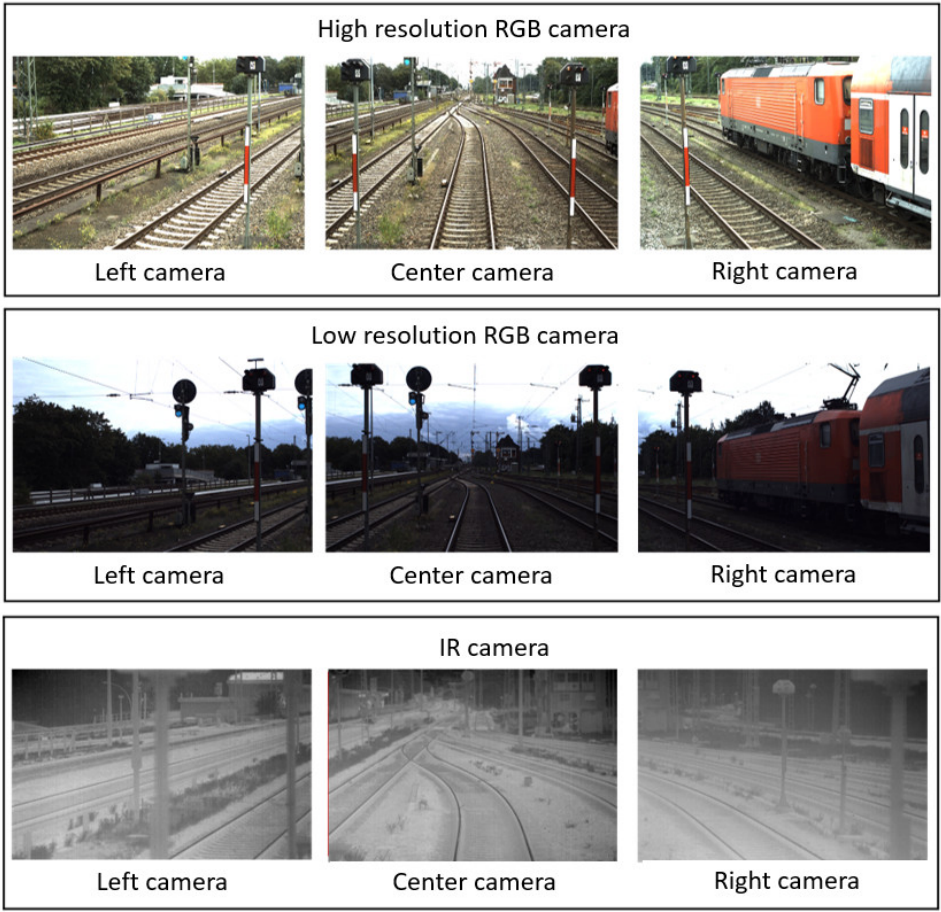
\includegraphics[width=0.5\textwidth]{images/datasets/db/2024-01-29 19_50_46-2305.03001}
\end{figure}



\section{RailSem dataset}



\chapter{Experiments} % 4000 words

\section{Modeling and performance evaluation} 



\section{Non-AI based segmentation}




\section{Deep-learning based segmentation}



\chapter{Results} % 2000 words





\chapter{Conclusion} % 500 words





Etwas Text... Hier kommen noch einige Abkürzunge vor zum Beispiel \ac{ABC},\ac{WWW} und \ac{ROFL}.


Literaturverweise sollten automatisch verwaltet werden, vor allem, wenn es viele Quellenverweise gibt. Beispiele sind  \cite{Ko05a}, \cite{Ko05b}, \cite{MiGo05}, \cite{TeGo14}, \cite{HuHa07}, \cite{HuZi10}, \cite{ZiKu07}, \cite{He07}, \cite{SIE11}, \cite{SIE14}, \cite{ISO98}, \cite{ATM11}, \cite{Hu11}, \cite{Po10}. Das verwendete Zitierformat (bzw.~das Format des Literaturverzeichnisses) ist entspechend der Vorgaben der Studiengänge zu wählen.



\section{Algorithms}


Use a defined environment for algorithms.

Algorithm \ref{alg:euclid} is an example from the gallery (\url{https://www.overleaf.com/latex/examples/euclids-algorithm-an-example-of-how-to-write-algorithms-in-latex/mbysznrmktqf}) .
%%%%%%%%%%%%%%%%%%%%%%%%%%%%%%%%%%%%%%%%%%%%%%%%%%%%%%%%%%%%%%%%%%
\begin{algorithm}
\caption{Euclid’s algorithm}\label{alg:euclid}
\begin{algorithmic}[1]
\Procedure{Euclid}{$a,b$}\Comment{The g.c.d. of a and b}
\State $r\gets a\bmod b$
\While{$r\not=0$}\Comment{We have the answer if r is 0}
\State $a\gets b$
\State $b\gets r$
\State $r\gets a\bmod b$
\EndWhile\label{euclidendwhile}
\State \textbf{return} $b$\Comment{The gcd is b}
\EndProcedure
\end{algorithmic}
\end{algorithm}
%%%%%%%%%%%%%%%%%%%%%%%%%%%%%%%%%%%%%%%%%%%%%%%%%%%%%%%%%%%%%%%%%% Hier beginnen die Verzeichnisse.
\clearpage                                                       % Beginne neue Seite

%\printbib                                                        % Literaturverzeichnis LaTeX-Zitier-Standard
%\printbib{Literatur}                                             % Literaturverzeichnis FH-Zitier-Standard
%\printbibliography
\bibliographystyle{plainnat} % We choose the "plain" reference style
\bibliography{Literatur} % Entries are in the refs.bib file

\clearpage

\listoffigures                                                   % Abbildungsverzeichnis
\clearpage

\listoftables                                                    % Tabellenverzeichnis
\clearpage

\listoflistings                                                  % Quellcodeverzeichnis
\clearpage

\phantomsection
\addcontentsline{toc}{chapter}{\listacroname}
\chapter*{\listacroname}
\begin{acronym}[XXXXX]
    \acro{ABC}[ABC]{Alphabet}
    \acro{WWW}[WWW]{world wide web}
    \acro{ROFL}[ROFL]{Rolling on floor laughing}
    
    
    
    \acro{ATO}[ATO]{Automatic Train Operations}
    \acro{CNN}[CNN]{Convolutional Neural Network}
    
\end{acronym}
%%%%%%%%%%%%%%%%%%%%%%%%%%%%%%%%%%%%%%%%%%%%%%%%%%%%%%%%%%%%%%%%%% Hier beginnt der Anhang.
\clearpage
\appendix
\chapter{Appendix A}
\clearpage
\chapter{Appendix B}
\end{document}
%%%%%%%%%%%%%%%%%%%%%%%%%%%%%%%%%%%%%%%%%%%%%%%%%%%%%%%%%%%%%%%%%% Ende des Inhalts